\documentclass{article}
\usepackage{graphicx}
\usepackage{epstopdf}
\usepackage{amsmath}
\usepackage[a4paper, total={7.5in, 10.5in}]{geometry}
\usepackage{hyperref}
\title{Mapping Cartesian Velocity to Compound-Angular Velocity}
\author{Jake Whitton}
\date{May 3rd, 2016}


\newcommand{\xdownarrow}[1]{%
  {\left\downarrow\vbox to #1{}\right.\kern-\nulldelimiterspace}
}

\newcommand\scalemath[2]{\scalebox{#1}{\mbox{\ensuremath{\displaystyle #2}}}}

\begin{document}
\maketitle
\section{Background}
I stumbled across this problem while trying to develop intuitive controls for a robotic arm, constructed for the science olympiad.  I find the solution to be very interesting, so I figured I would give my shot at basic LaTex and try writing up a proof of my solution.
\\
\\
The problem can be summed up with the following picture.
\\
\\
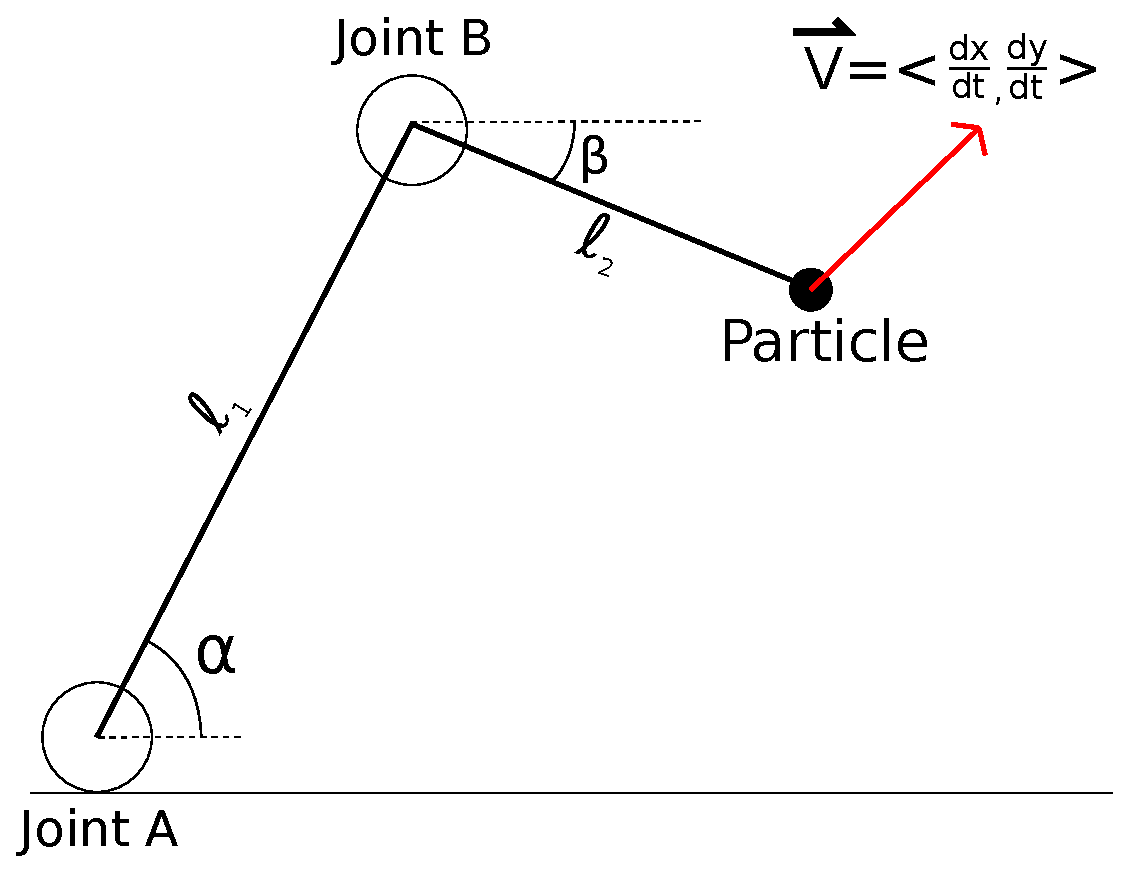
\includegraphics[width=\textwidth]{drawing1.eps}
\\
\\
The angle Joint A makes with the horizontal is denoted $\alpha$.  The angle Joint B makes with the Horizontal is denoted $\beta$.
\\
\\
Joint A is fixed in space, but allowed to rotate freely.  Joint B's position is dependent upon the current value of $\alpha$, and can similarly rotate freely.
\\
\\
At the end of the compound arm, there is a particle that is moving with a cartesian velocity $\vec{v}$.
\begin{equation*}
\vec{v} = \langle\frac{dx}{dt}, \frac{dy}{dt}\rangle
\end{equation*}
\\
The two lengths of the compound arm, in the interest of generality, have been left to $\ell_1$ and $\ell_2$.
\\
\\
We can represent the independent angular velocities of Joint A and Joint B with a two-dimensional vector like so:
\begin{equation*}
\vec{\omega} = \langle \frac{d\alpha}{dt}, \frac{d\beta}{dt} \rangle
\end{equation*}


\section{Problem}
Develop a mapping function, using reasonable parameters, that will return the current angular velocity vector $\vec{\omega}$ that should be used such that the particle moves with a cartesian velocity $\vec{v}$
\\
\begin{equation*}
M \to \vec{\omega} = M(\frac{dx}{dt}, \frac{dy}{dt}, ...) 
\end{equation*}
\\
\section{Solution}
Getting more triggy with it, we can represent the figure as two right triangles like the following:
\\
\\
\\
\\
\\
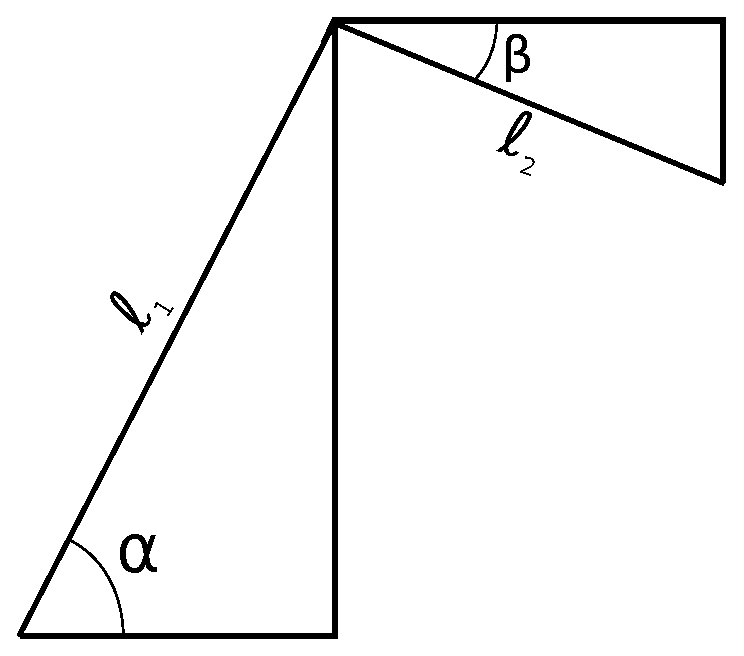
\includegraphics[width=450pt]{drawing2.eps}
\\
\\
Because we are all so good at trig, we can give the legs of these triangles in terms of $\ell_1$, $\ell_2$, $\alpha$, and $\beta$.
\\
\\
\\
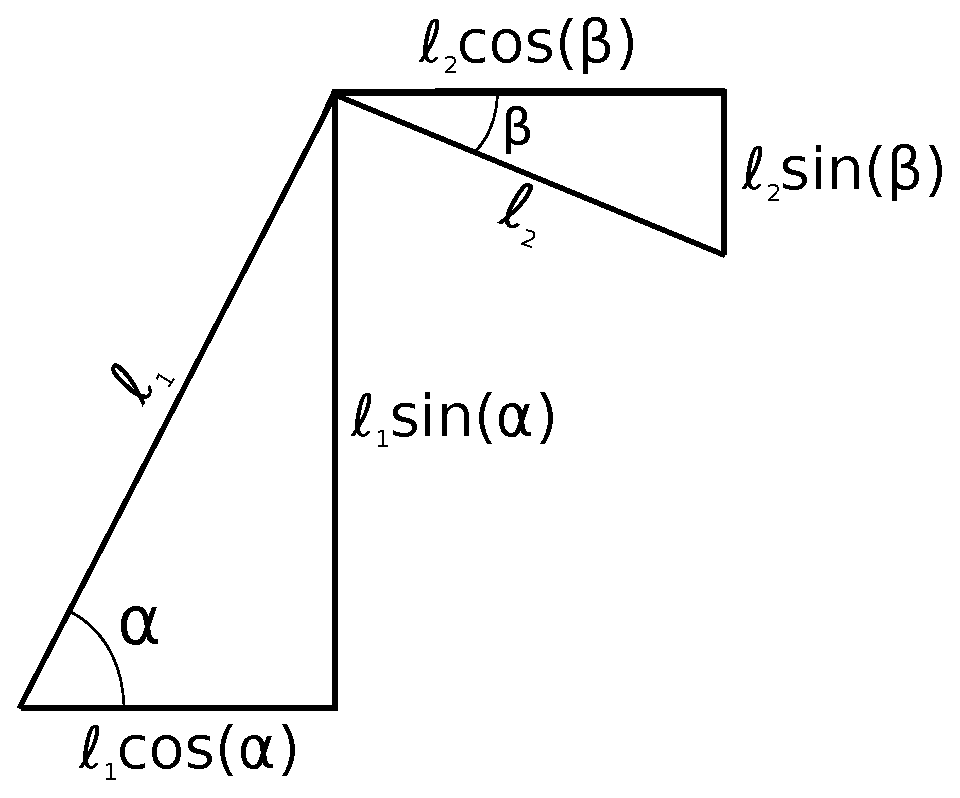
\includegraphics[width=\textwidth]{drawing3.eps}
\\
\\
\\
\\
Now, it is abundantly clear that
\\
\\
\begin{equation} \label{position}
\langle x, y \rangle = \langle \ell_1cos(\alpha) + \ell_2cos(\beta), \ell_1sin(\alpha) + \ell_2sin(\beta) \rangle
\end{equation}
\\
\\
Differentiating, we get
\\
\\
\begin{equation*}
\frac{d}{dt}[\langle x, y \rangle] = \frac{d}{dt}[\langle \ell_1cos(\alpha) + \ell_2cos(\beta), \ell_1sin(\alpha) + \ell_2sin(\beta) \rangle]
\end{equation*}
\\
\begin{equation}
\langle \frac{dx}{dt}, \frac{dy}{dt} \rangle = \langle -\ell_1sin(\alpha)\frac{d\alpha}{dt} - \ell_2sin(\beta)\frac{d\beta}{dt}, \ell_1cos(\alpha)\frac{d\alpha}{dt} + \ell_2cos(\beta)\frac{d\beta}{dt} \rangle
\end{equation}
Writing that result in terms of a system of equations, we get
\\
\begin{align*}
-\ell_1sin(\alpha)\frac{d\alpha}{dt} - \ell_2sin(\beta)\frac{d\beta}{dt} = \frac{dx}{dt}\\
\ell_1cos(\alpha)\frac{d\alpha}{dt} + \ell_2cos(\beta)\frac{d\beta}{dt} = \frac{dy}{dt}\\
\end{align*}
\\
Or, in matrix notation
\\
\begin{equation}
\begin{bmatrix}
-\ell_1sin(\alpha) & -\ell_2sin(\beta)\\\\
\ell_1cos(\alpha) & \ell_2cos(\beta)
\end{bmatrix}
\begin{bmatrix}
\frac{d\alpha}{dt}\\\\
\frac{d\beta}{dt}
\end{bmatrix}
=
\begin{bmatrix}
\frac{dx}{dt}\\\\
\frac{dy}{dt}
\end{bmatrix}
\end{equation}
\\
\\
In order to solve this, we can use Reduced Row-Echelon Form(RREF).
\begin{equation}
RREF(
\begin{bmatrix}
-\ell_1sin(\alpha) & -\ell_2sin(\beta) & \frac{dx}{dt}\\\\
\ell_1cos(\alpha) & \ell_2cos(\beta) & \frac{dy}{dt}
\end{bmatrix}
)
\end{equation}
\\
\\
In order to do this clearly, I will define some notation.
\begin{itemize}
\item Transpose$_{ab}$ 	means swap row a and row b.
\item Multiply$_a(k)$ 	means multiply row a by a scalar $k$.
\item Add$_{ab}(k)$ 	means scale row a by a scalar $k$, and add that to b.  Note: does not change row a.  It only uses it for the calculation.
\end{itemize}
We start with our unmodified augmented matrix
\\

%Beginning of RREF
\begin{equation*}
\begin{bmatrix}
-\ell_1sin(\alpha) & -\ell_2sin(\beta) & \frac{dx}{dt}\\\\
\ell_1cos(\alpha) & \ell_2cos(\beta) & \frac{dy}{dt}
\end{bmatrix}
\end{equation*}
\begin{center}
	\centering
	$\downarrow{Multiply_1(cos(\alpha)), Multiply_2(sin(\alpha))}$
\end{center}

\begin{equation*}
\begin{bmatrix}
-\ell_1sin(\alpha)cos(\alpha) & -\ell_2cos(\alpha)sin(\beta) & \frac{dx}{dt}cos(\alpha)\\\\
\ell_1sin(\alpha)cos(\alpha) & \ell_2sin(\alpha)cos(\beta) & \frac{dy}{dt}sin(\alpha)
\end{bmatrix}
\end{equation*}
\begin{center}
	\centering
	$\downarrow{Add_{12}(1)}$
\end{center}

\begin{equation*}
\begin{bmatrix}
-\ell_1sin(\alpha)cos(\alpha) & -\ell_2cos(\alpha)sin(\beta) & \frac{dx}{dt}cos(\alpha)\\\\
0 & \ell_2sin(\alpha)cos(\beta) -\ell_2cos(\alpha)sin(\beta) & \frac{dy}{dt}sin(\alpha) + \frac{dx}{dt}cos(\alpha)
\end{bmatrix}
\end{equation*}
\begin{center}
	\centering
	$\downarrow{Simplify}$
\end{center}

\begin{equation*}
\begin{bmatrix}
-\ell_1sin(\alpha)cos(\alpha) & -\ell_2cos(\alpha)sin(\beta) & \frac{dx}{dt}cos(\alpha)\\\\
0 & \ell_2\big[sin(\alpha)cos(\beta) -cos(\alpha)sin(\beta)\big] & \frac{dy}{dt}sin(\alpha) + \frac{dx}{dt}cos(\alpha)
\end{bmatrix}
\end{equation*}
\begin{center}
	\centering
	$\downarrow{Multiply_1(\frac{sin(\alpha)cos(\beta) -cos(\alpha)sin(\beta)}{cos(\alpha)sin(\beta)})}$
\end{center}

\begin{equation*}
\begin{bmatrix}
\frac{-\ell_1sin(\alpha)cos(\alpha)\big[sin(\alpha)cos(\beta) -cos(\alpha)sin(\beta)\big]}{cos(\alpha)sin(\beta)} & -\ell_2\big[sin(\alpha)cos(\beta) -cos(\alpha)sin(\beta)\big] & \frac{\frac{dx}{dt}cos(\alpha)\big[sin(\alpha)cos(\beta) -cos(\alpha)sin(\beta)\big]}{cos(\alpha)sin(\beta)}\\\\
0 & \ell_2\big[sin(\alpha)cos(\beta) -cos(\alpha)sin(\beta)\big] & \frac{dy}{dt}sin(\alpha) + \frac{dx}{dt}cos(\alpha)
\end{bmatrix}
\end{equation*}
\begin{center}
	\centering
	$\downarrow{Simplify}$
\end{center}

\begin{equation*}
\begin{bmatrix}
\frac{-\ell_1sin(\alpha)\big[sin(\alpha)cos(\beta) -cos(\alpha)sin(\beta)\big]}{sin(\beta)} & -\ell_2\big[sin(\alpha)cos(\beta) -cos(\alpha)sin(\beta)\big] & \frac{\frac{dx}{dt}\big[sin(\alpha)cos(\beta) -cos(\alpha)sin(\beta)\big]}{sin(\beta)}\\\\
0 & \ell_2\big[sin(\alpha)cos(\beta) -cos(\alpha)sin(\beta)\big] & \frac{dy}{dt}sin(\alpha) + \frac{dx}{dt}cos(\alpha)
\end{bmatrix}
\end{equation*}
\begin{center}
	\centering
	$\downarrow{Add_{21}(1)}$
\end{center}

\begin{equation*}
\begin{bmatrix}
\frac{-\ell_1sin(\alpha)\big[sin(\alpha)cos(\beta) -cos(\alpha)sin(\beta)\big]}{sin(\beta)} & 0 & \frac{\frac{dx}{dt}\big[sin(\alpha)cos(\beta) -cos(\alpha)sin(\beta)\big]}{sin(\beta)} + \frac{dy}{dt}sin(\alpha) + \frac{dx}{dt}cos(\alpha)\\\\
0 & \ell_2\big[sin(\alpha)cos(\beta) -cos(\alpha)sin(\beta)\big] & \frac{dy}{dt}sin(\alpha) + \frac{dx}{dt}cos(\alpha)
\end{bmatrix}
\end{equation*}
\begin{center}
	\centering
	$\downarrow{Multiply_1(\frac{sin(\beta)}{-\ell_1sin(\alpha)\big[sin(\alpha)cos(\beta) -cos(\alpha)sin(\beta)\big]}), Multiply_2(\frac{1}{\ell_2\big[sin(\alpha)cos(\beta) -cos(\alpha)sin(\beta)\big]})}$
\end{center}

\begin{equation*}
\begin{bmatrix}
1 & 0 & \frac{sin(\beta)}{-\ell_1sin(\alpha)\big[sin(\alpha)cos(\beta) -cos(\alpha)sin(\beta)\big]}\bigg[\frac{\frac{dx}{dt}\big[sin(\alpha)cos(\beta) -cos(\alpha)sin(\beta)\big]}{sin(\beta)} + \frac{dy}{dt}sin(\alpha) + \frac{dx}{dt}cos(\alpha)\bigg]\\\\
0 & 1 & \frac{1}{\ell_2\big[sin(\alpha)cos(\beta) -cos(\alpha)sin(\beta)\big]}\bigg[\frac{dy}{dt}sin(\alpha) + \frac{dx}{dt}cos(\alpha)\bigg]
\end{bmatrix}
\end{equation*}
\begin{center}
	\centering
	$\downarrow{Simplify}$
\end{center}

\begin{equation}
\begin{bmatrix}
1 & 0 & -\frac{1}{\ell_1sin(\alpha)}\bigg[\frac{dx}{dy} + sin(\beta)\frac{\frac{dy}{dt}sin(\alpha) + \frac{dx}{dt}cos(\alpha)}{sin(\alpha)cos(\beta) -cos(\alpha)sin(\beta)}\bigg]\\\\
0 & 1 & \frac{1}{\ell_2}\bigg[\frac{\frac{dy}{dt}sin(\alpha) + \frac{dx}{dt}cos(\alpha)}{sin(\alpha)cos(\beta) -cos(\alpha)sin(\beta)}\bigg]
\end{bmatrix}
\end{equation}
\\
Thus,
\\
\begin{equation}
\begin{bmatrix}
\frac{d\alpha}{dt}\\\\
\frac{d\beta}{dt}
\end{bmatrix}=
\begin{bmatrix}
-\frac{1}{\ell_1sin(\alpha)}\bigg[\frac{dx}{dy} + sin(\beta)\frac{\frac{dy}{dt}sin(\alpha) + \frac{dx}{dt}cos(\alpha)}{sin(\alpha)cos(\beta) -cos(\alpha)sin(\beta)}\bigg]\\\\
\frac{1}{\ell_2}\bigg[\frac{\frac{dy}{dt}sin(\alpha) + \frac{dx}{dt}cos(\alpha)}{sin(\alpha)cos(\beta) -cos(\alpha)sin(\beta)}\bigg]
\end{bmatrix}
\end{equation}
\\
\\
Or, equivalently,
\\
\begin{equation}
\vec{\omega}(\alpha, \beta, \frac{dx}{dt}, \frac{dy}{dt}) = \langle -\frac{1}{\ell_1sin(\alpha)}\bigg[\frac{dx}{dy} + sin(\beta)\frac{\frac{dy}{dt}sin(\alpha) + \frac{dx}{dt}cos(\alpha)}{sin(\alpha)cos(\beta) -cos(\alpha)sin(\beta)}\bigg], \frac{1}{\ell_2}\bigg[\frac{\frac{dy}{dt}sin(\alpha) + \frac{dx}{dt}cos(\alpha)}{sin(\alpha)cos(\beta) -cos(\alpha)sin(\beta)}\bigg] \rangle
\end{equation}
\\
\\
And, with that, the problem is solved.  It stands to reason that the expression for $\frac{d\alpha}{dt}$ would be more complicated, since any change in $\alpha$ would also change the position of Joint B.
\section{Shortcomings of the Model}
This model isn't entirely perfect.  There are some cases when the function fails to return a meaningful value.
\\
\\
Consider the motif
\begin{equation*}
sin(\alpha)cos(\beta) -cos(\alpha)sin(\beta)
\end{equation*}
\\
If $\alpha$ was equal to $\beta$, that expression would return 0, which is a problem, because that motif is in the denominator of both vector components of $\vec{\omega}$.
\\
Consider the case in which both $\alpha$ and $\beta$ were equal to $\frac{\pi}{4}$ radians.  Also assume that $\vec{v} = \langle1,1\rangle$.  It is intuitively obvious that $\vec{\omega}$ should not exist, since you can't push the particle outside of the locus of points which the arm can inhabit.  Your locus of potential points is just the semi-circle of radius $\ell_1 + \ell_2$.  However, doesn't check to see what direction $\vec{v}$ is pointing.  Whenever $\alpha = \beta$, the function fails to return a meaningful result.
\\
\\
When implementing this model in code, you can account for this, by always making sure to check if $\alpha = \beta$ before calling the function.  Then, it is likely that it will return a real-valued vector.  You can always scale the vector down proportionally if it is too fast for your motors.
\\
\\
Similarily, if $sin(\alpha)$ is 0, the $\frac{d\alpha}{dt}$ will fail to compute, since $sin(\alpha)$ is in the denominator of the first vector component of $\vec{\omega}$
\\
\\
Again, when implementing this with code, we can take care of these special cases at runtime.  For the majority of the time, though, this model works really well.
\\
\\
If you have any questions, you can email me at Jakewhitton@Yahoo.com.  If you would like to see the code that implements this for a robotics application, you can visit \url{https://github.com/jakewhitton/robotarm}.
\end{document}